\documentclass[twocolumn, ]{article}
\usepackage{amsmath}
\usepackage{graphicx}

\usepackage{geometry}
 \geometry{
 a4paper,
 total={170mm,257mm},
 left=5mm,
right=5 mm,
bottom=5 mm,
 top=5mm,
 }
 \usepackage{setspace}
\setstretch{0.3}

\begin{document}

\section*{\small Cheat Sheet for EE463}

\subsection*{\small Performance Parameters}
\begin{equation*}
Form Factor=\frac{V_{rms}}{V_{avg}}
\end{equation*}
\begin{equation*}
Crest Factor=\frac{V_{peak}}{V_{rms}}
\end{equation*}
\begin{equation*}
Distortion Factor=\frac{I_{1rms}}{I_{rms}}
\end{equation*}
\textit{$\phi$ : phase difference between fundamentals of current and voltage}
\begin{equation*}
Displacement Power Factor=\cos(\phi)
\end{equation*}
\begin{equation*}
True Power Factor=\frac{P}{S}=DPF \frac{I_{1,RMS}}{I_{RMS}}
\end{equation*}
\begin{equation*}
THD=\sqrt{(\frac{I_{rms}}{I_{1rms}})^2-1}
\end{equation*}



  \begin{figure}[!ht]
	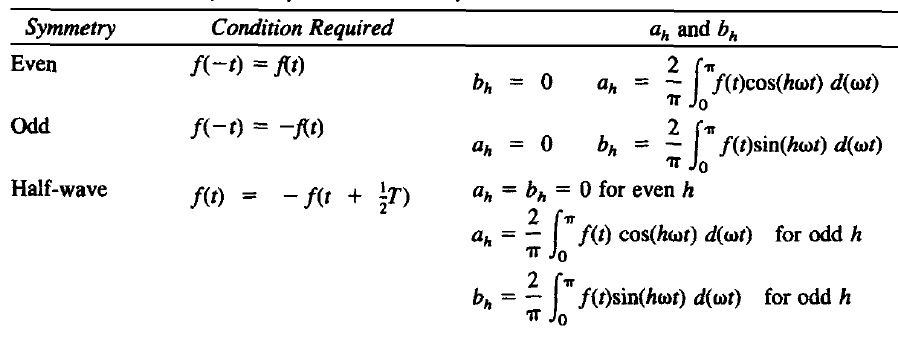
\includegraphics[scale=0.30]{Fourier.png}
	\caption{Fourier Transform Table}
\end{figure}

\begin{figure}[!ht]
	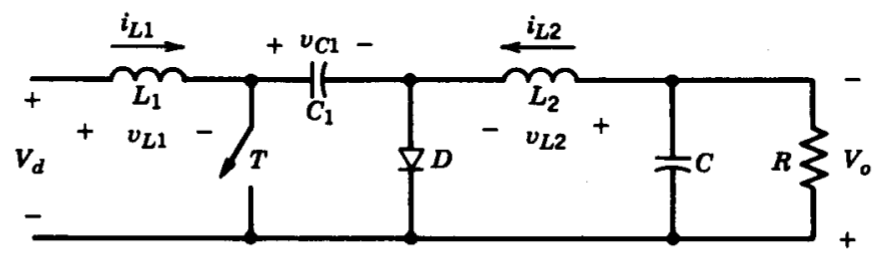
\includegraphics[scale=0.20]{cuk_converter.png}
	\caption{Cuk converter}
\end{figure}

\begin{figure}[!ht]
	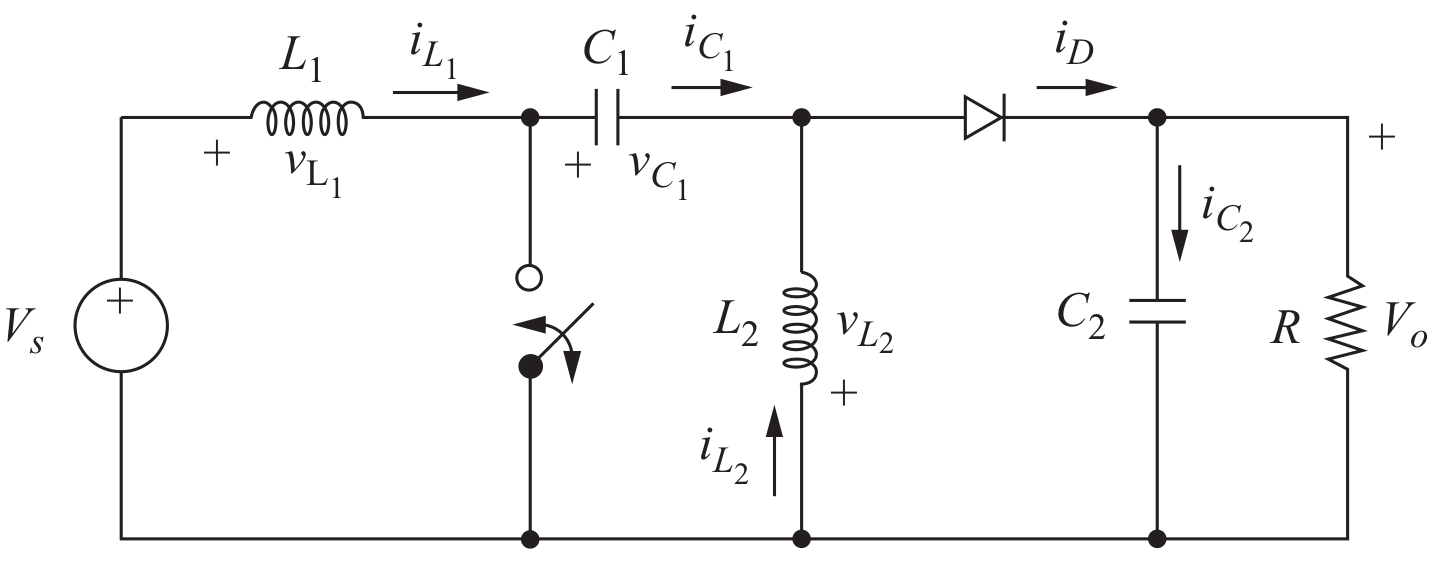
\includegraphics[width=2.5in,height=1in]{sepic_operation.png}
	\caption{Sepic converter}
\end{figure}

\begin{figure}[!ht]
	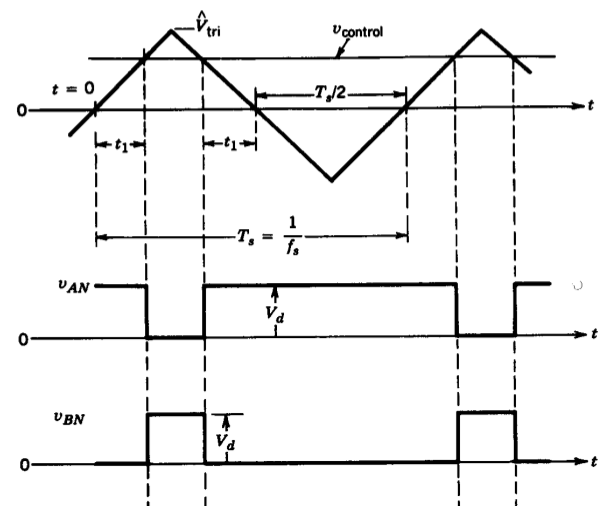
\includegraphics[width=2.5in,height=1in]{bipolar1.png}
	\caption{Bipolar Switching}
\end{figure}
\begin{figure}[!ht]
	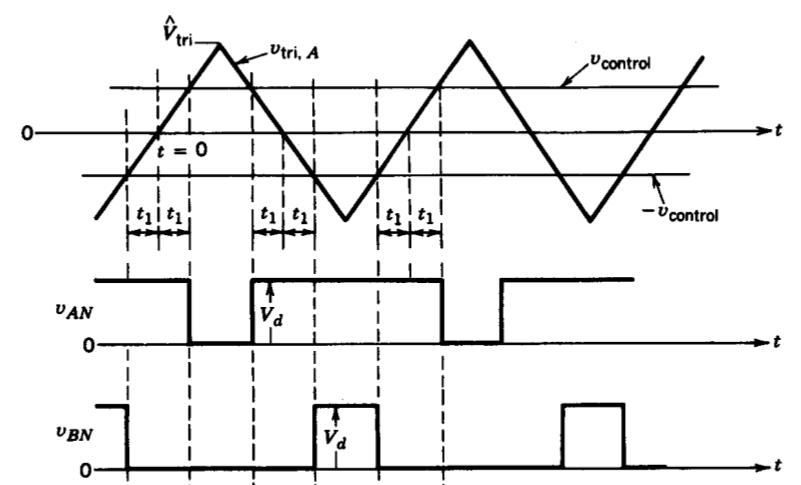
\includegraphics[width=2.5in,height=1in]{unipolar1.png}
	\caption{Unipolar switching}
\end{figure}








\end{document}
